\documentclass[IN,english]{tumbook}
\usepackage{tabularx}
%\usepackage[utf8]{inputenc}
%\usepackage[T1]{fontenc}
%\usepackage{graphicx}
%\usepackage{amsmath}

\makeindex

% Information for the title page
\Seminar{Software Engineering for Business Applications - Master}
\Semester{SS 2015}
\title{Business Model for the Web Application \emph{Travel Diary}}
\Untertitel{}
\Themensteller{Prof. Dr. Florian Matthes}
\Autorenadresse{}
\Matrikelnummer{}
\Fachsemester{}
\Abgabetermin{13. May 2015}
\author{Chetan Basuray, Mantosh Kumar, Ulrike Niemann, Albert Steckermeier}
\date{13. May 2015}



\begin{document}

\maketitle
\newpage
\tableofcontents
\newpage

\chapter{Introduction}

In order to operate the \emph{Travel Diary} web application some form of revenue is required to establish and sustain the service. For that purpose this paper describes the business model in the structure of the business model canvas depicted in the next section.

\chapter{Business Model Canvas}

\begin{center}
	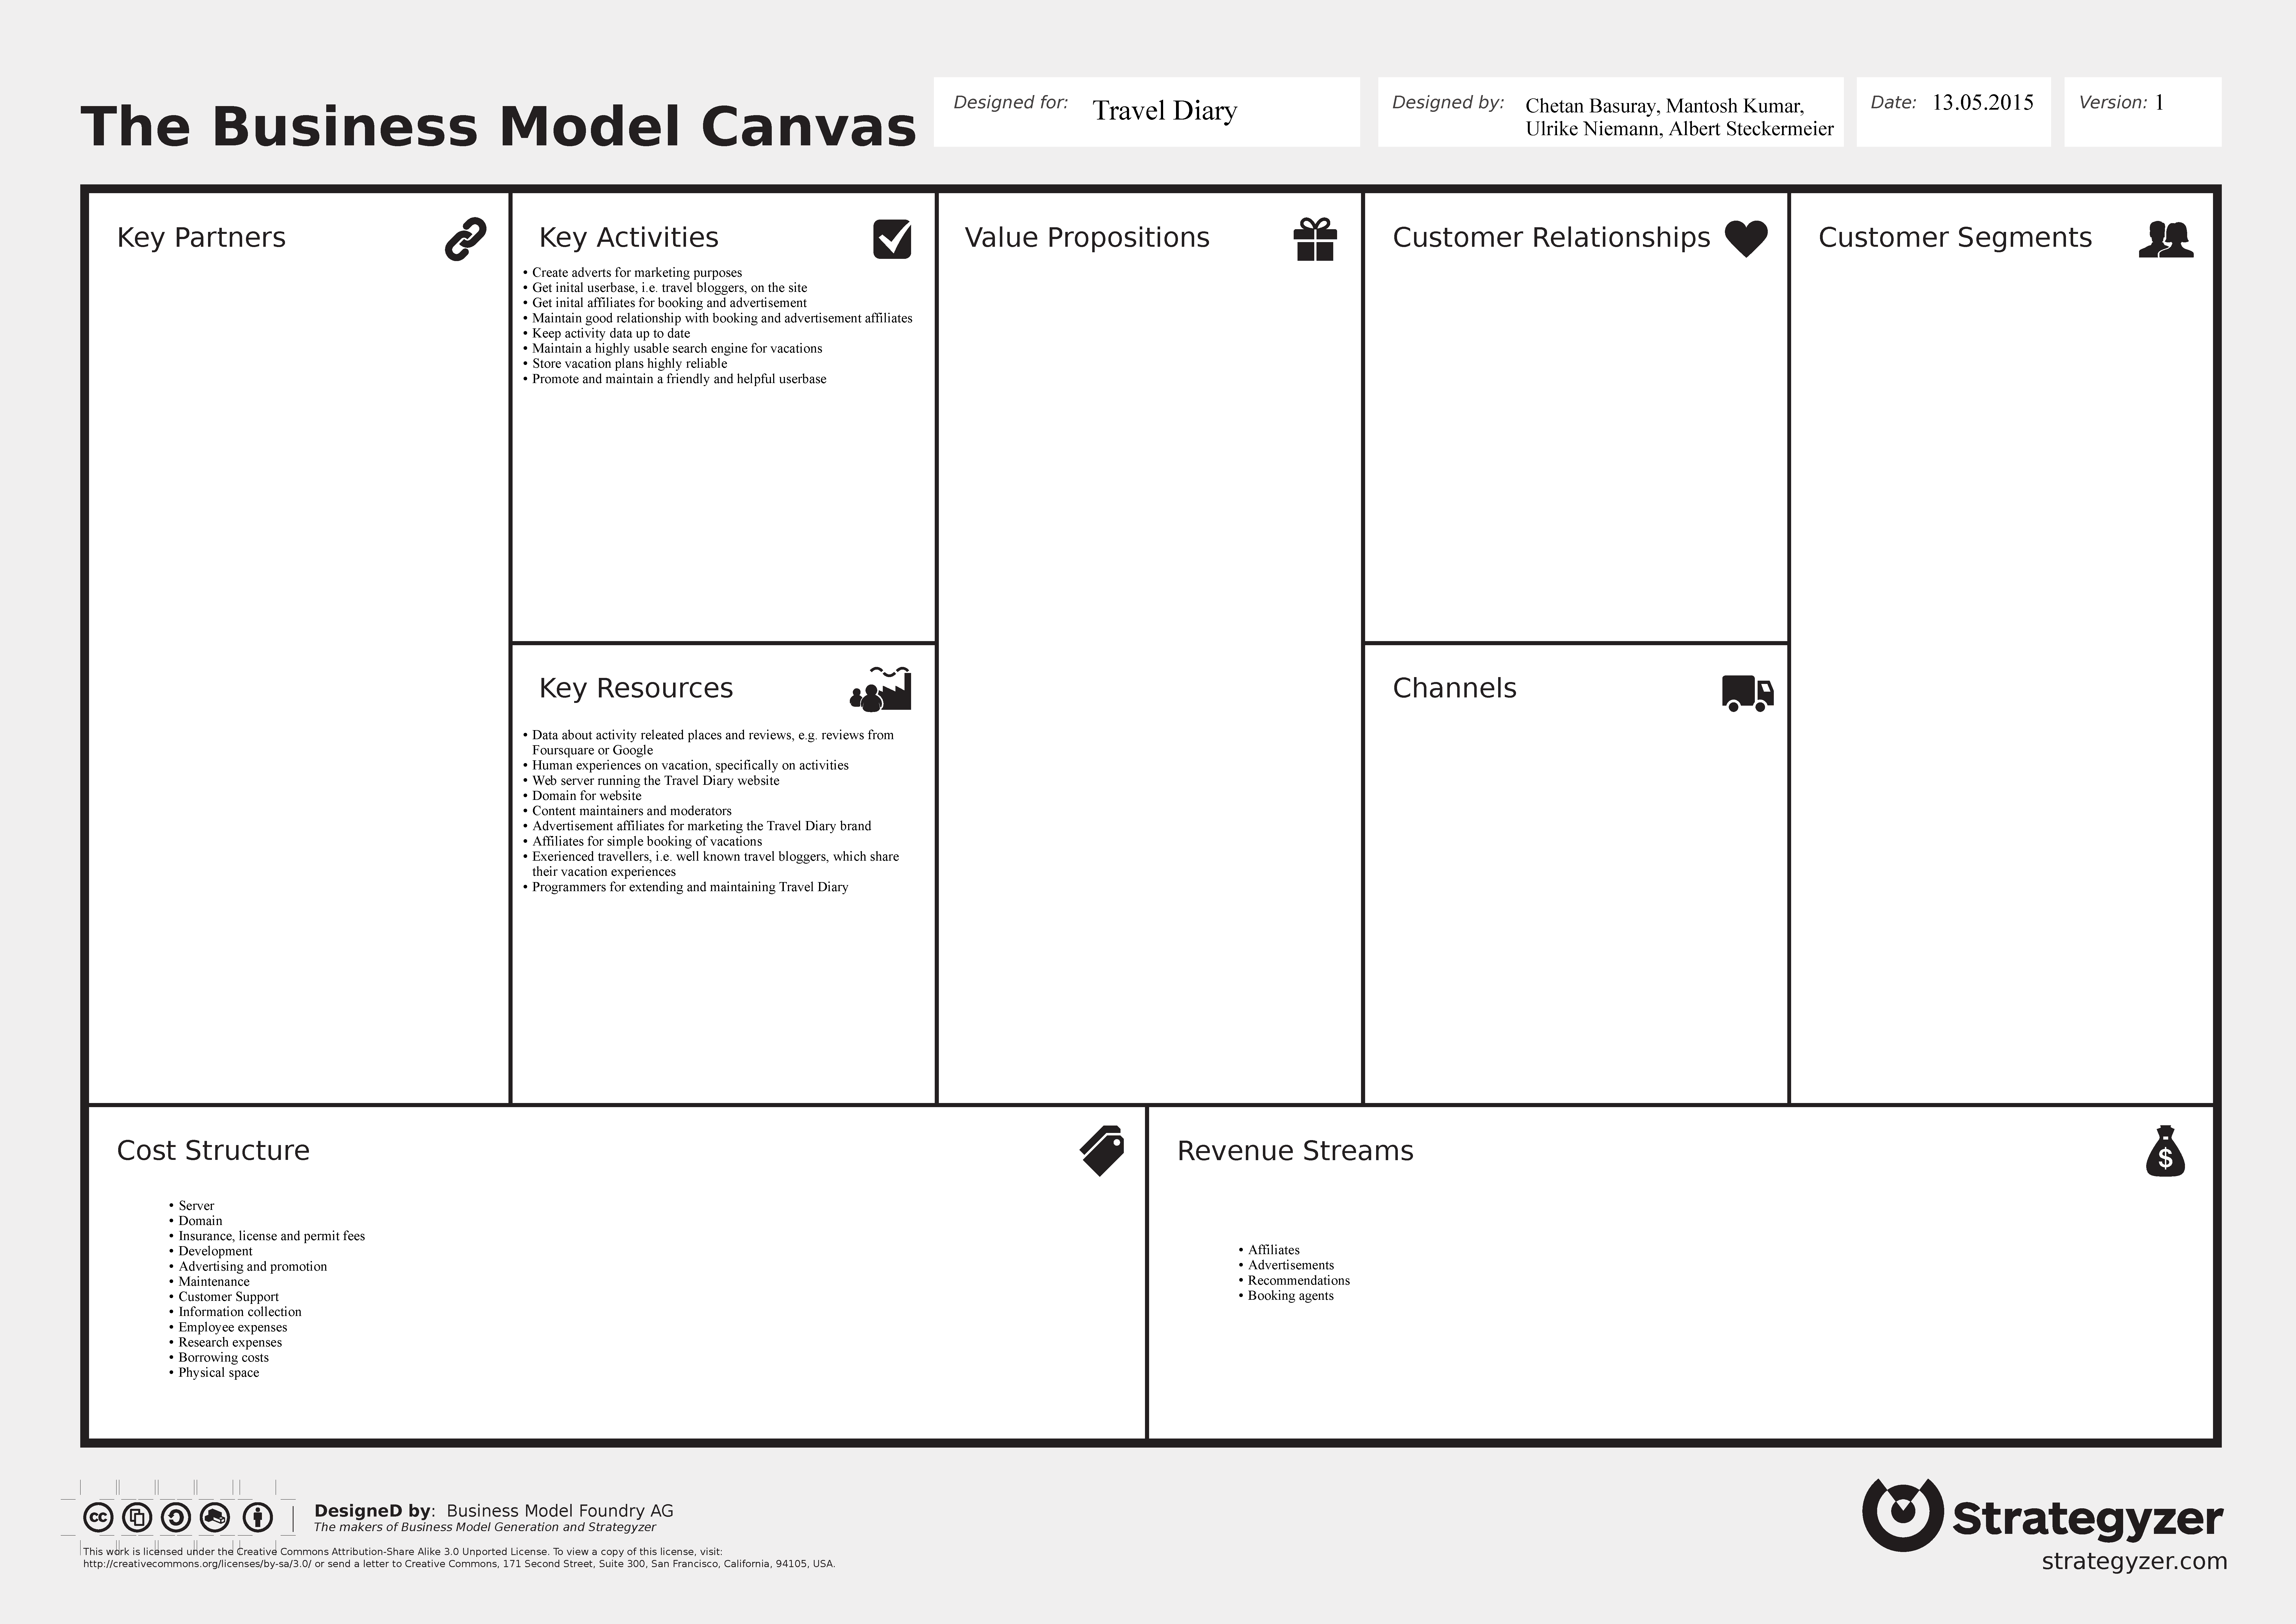
\includegraphics[scale=0.17, angle=90]{graphics/team-39-exercise-2-business-model-canvas}
\end{center}

\chapter{Business Model}

\section{Value Proposition}

\section{Customer Segment}

\section{Customer Relationships}


Customer relationship entails all aspects of interaction that a company has with its customers. The principle benefit includes a 360-degree view of what customers and the general market want, and using this information to enhance your application.

Travel Diary has several categories of customer relationships.

\begin{enumerate}
\item Co-creation - The application invites customers to write reviews, share his/her trip experience and thus co-produce business and values for itself and the customers. In real sense, customers are the true champions of this application. This is Travel Diary primary and utmost important relationship with customers.
\item Self-service - No direct relationship with customer, everything is provided to them to help themselves in FAQ section. 
\item Personal assistance - This is based on human interaction. The customer can communicate with a real customer representative over chat or phone. This will obviously cost some money but is manageable as for Travel Diary most of the purposes are served by above two relationships.
\end{enumerate}

\section{Channels}

Channels are how a company reaches its Customer Segments to deliver a Value Proposition.There is a growing interest in social procurement. To reach out to the mass Travel Diary is planning to use web, social networks and blogging extensively. Travel Diary is going to exhibit the experiences shared by its users as an evidence of its excellent service. Although travel agencies are its direct competitors but it plans to partner with these agencies. For customer support, there will be several segments that will address customer's queries.

\section{Key Partners}

\section{Key Activities}

Next the necessary key activities that keep the Travel Diary service going will be discussed. First continuous advertising has to be implemented. The advertisement needs to be redesigned and distributed continually to fit current customer interests. Affiliate sites related to traveling will be used to advertise the Travel Diary service. Good advertisement should get an initial user base on the site. Especially travel bloggers need to be targeted in advertisement to get enough content creators on the site.

Besides advertisement, connections to affiliates for the booking of vacations have to be established. Sites like booking.com will be targeted as affiliates. When the relationships with affiliates are established they also have to cultivated. For that purpose regular feedback and personal meetings should be set up regularly. With the affiliates the infrastructure for the service is provided but there are some maintenance activities necessary to stay competitive.
With the help of travel bloggers as content creators a large part of the maintained activity data, i.e. related reviews and locations, should be kept up to date. In general moderation of content is probably necessary. Moderation means removing deprecated user created data and reviewing user created content in terms of usefulness and sensible content. All of this should be done with the goal of creating a friendly and helpful community of travelers in mind. Consequently the quality of data that can be searched and re-used is higher which draws more users to the service. To achieve an effective search that really yields the best possible results, the search engine has to be refined continually to achieve great search results and stand out amongst competitors.

Because data loss is always a big hassle the service should also be run on a redundant platform to minimize the risk. This could however be delegated to the provider of the servers running Travel Diary.

\section{Key Resources}

All of the activities above require some key resources to maintain the service. Affiliates for advertisement and booking will be required as can easily be seen when looking at the activities above. Also moderators, content maintainers and programmers will be needed to deal with users requests, user problems, bugs and the operation of the service.

Furthermore Travel Diary relies heavily on data about possible activities which has to be gathered or made accessible in some form. The data will be in the form of reviews which give a rough idea of the activity or place related to it. Such data could be acquired from Google Maps or Foursquare. From these sites a lot of data can be reused for the Travel Diary service and will be enriched further by user created content. Here it is also clear that human experiences on vacation will be the enriching factor which will be one of the key data resources. A lot of experience comes from travel bloggers which will be one of the main human resource the service will require. 

Lastly of course the Domain as well as the web server running Travel Diary are vital resources.

\section{Cost Structure}

The cost structure for the business model is quite simple. We will need to have sufficient funds for a server and a domain. We would also need to have some insurance. A license and permit fees may be needed depending upon the type of transactions we do and whether we need to use some proprietary software. Cost for development and maintenance of the entire project also needs to be considered and in the long run this may also include developer fees. A big part of the expenses will be advertisements. We will need a lot of experienced writers to collect information for our site and that will be expensive. Building some sort of a customer support section, either through facebook and emails or through phones will also need to be financed. Finally salary to be paid for the employees, either developers or otherwise will come into consideration. We will also need some expenses for researching the field we are moving into and constant research is always needed to stay ahead of competition. Finally investment will mostly come through borrowing money and there will be expenses incurred when we pay interests. Also, in future, a demand for larger physical spaces will arise and that will need to be paid for as well.

\section{Revenue Streams}

The most important revenue streams for our website will definitely be the affiliates through which we will provide booking facilities to a customer. Directed advertisements, like those provided by google adwords, will also be an important source of revenue. Customers are willing to pay for recommendations and booking agents. By combining these two in our idea, we will be able to generate revenue since we aim to provide personalized recommendations and bookings for those.

\section{Conclusion}

To sum up, the business model is heavily based on the affiliate model. 

\chapter{Contribution}

\begin{table}
	\begin{tabularx}{\textwidth}{|>{\setlength\hsize{\hsize}\setlength\linewidth{\hsize}}X|>{\setlength\hsize{\hsize}\setlength\linewidth{\hsize}}X|}
		\hline
		\multicolumn{1}{|c|}{Contributor} & \multicolumn{1}{|c|}{Contribution} \\
		\hline
		Chetan Basuray & 
		\begin{itemize}
			\item Wrote Cost Structure
			\item Wrote Revenue Streams
		\end{itemize} \\
		\hline
		Mantosh Kumar & 
		\begin{itemize}
			\item Wrote Channels
			\item Wrote Customer Relationship
		\end{itemize} \\
		\hline
		Ulrike Niemann & 
		\begin{itemize}
			\item Wrote Key Partners
			\item Wrote Value Propositions
			\item Wrote Customer Segment
		\end{itemize} \\
		\hline
		Albert Steckermeier  & 
		\begin{itemize}
			\item Wrote Introduction
			\item Wrote Key Activities
			\item Wrote Key Resources
			\item Wrote Conclusion
		\end{itemize}
		\\
		\hline
	\end{tabularx}
	\label{tab:contribution}
	\caption{Individual contribution of the team members to this paper.}
\end{table}
\end{document}